\documentclass[10pt,a4paper,english]{article}
\usepackage{babel}
\usepackage{ae}
\usepackage{aeguill}
\usepackage{shortvrb}
\usepackage[latin1]{inputenc}
\usepackage{tabularx}
\usepackage{longtable}
\setlength{\extrarowheight}{2pt}
\usepackage{amsmath}
\usepackage{graphicx}
\usepackage{color}
\usepackage{multirow}
\usepackage{float}\usepackage{ifthen}
\usepackage[DIV12]{typearea}
% generated by Docutils <http://docutils.sourceforge.net/>
\newlength{\admonitionwidth}
\setlength{\admonitionwidth}{0.9\textwidth}
\newlength{\docinfowidth}
\setlength{\docinfowidth}{0.9\textwidth}
\newlength{\locallinewidth}
\newcommand{\optionlistlabel}[1]{\bf #1 \hfill}
\newenvironment{optionlist}[1]
{\begin{list}{}
  {\setlength{\labelwidth}{#1}
   \setlength{\rightmargin}{1cm}
   \setlength{\leftmargin}{\rightmargin}
   \addtolength{\leftmargin}{\labelwidth}
   \addtolength{\leftmargin}{\labelsep}
   \renewcommand{\makelabel}{\optionlistlabel}}
}{\end{list}}
\newlength{\lineblockindentation}
\setlength{\lineblockindentation}{2.5em}
\newenvironment{lineblock}[1]
{\begin{list}{}
  {\setlength{\partopsep}{\parskip}
   \addtolength{\partopsep}{\baselineskip}
   \topsep0pt\itemsep0.15\baselineskip\parsep0pt
   \leftmargin#1}
 \raggedright}
{\end{list}}
% begin: floats for footnotes tweaking.
\setlength{\floatsep}{0.5em}
\setlength{\textfloatsep}{\fill}
\addtolength{\textfloatsep}{3em}
\renewcommand{\textfraction}{0.5}
\renewcommand{\topfraction}{0.5}
\renewcommand{\bottomfraction}{0.5}
\setcounter{totalnumber}{50}
\setcounter{topnumber}{50}
\setcounter{bottomnumber}{50}
% end floats for footnotes
% some commands, that could be overwritten in the style file.
\newcommand{\rubric}[1]{\subsection*{~\hfill {\it #1} \hfill ~}}
\newcommand{\titlereference}[1]{\textsl{#1}}
% end of "some commands"
\ifthenelse{\isundefined{\hypersetup}}{
\usepackage[colorlinks=true,linkcolor=blue,urlcolor=blue]{hyperref}
}{}
\title{dot2tex - A Graphviz to LaTeX converter}
\author{}
\date{}
\hypersetup{
pdftitle={dot2tex - A Graphviz to LaTeX converter},
pdfauthor={Kjell Magne Fauske}
}
\raggedbottom
\begin{document}
\maketitle
%___________________________________________________________________________
\begin{center}
\begin{tabularx}{\docinfowidth}{lX}
\textbf{Author}: &
	Kjell Magne Fauske \\
\textbf{Version}: &
	2.7.0 \\
\textbf{Licence}: &
	MIT \\
\end{tabularx}
\end{center}

\setlength{\locallinewidth}{\linewidth}


Dot2tex is a tool for converting graphs generated by \href{http://www.graphviz.org/}{Graphviz} to formats suitable for use with LaTeX. Currently dot2tex can generate code for use with \href{http://tug.org/PSTricks/main.cgi/}{PSTricks} and \href{http://www.ctan.org/tex-archive/help/Catalogue/entries/pgf.html}{PGF/TikZ}.

The purpose of dot2tex is to give graphs a more LaTeX look and feel. This is accomplished by:
\begin{itemize}
\item {} 
Typesetting labels with LaTeX, allowing mathematical notation.

\item {} 
Using native \href{http://tug.org/PSTricks/main.cgi/}{PSTricks} and \href{http://www.ctan.org/tex-archive/help/Catalogue/entries/pgf.html}{PGF/TikZ} commands for drawing arrows, edges
and nodes.

\item {} 
Using output specific styles to customize the output.

\end{itemize}


%___________________________________________________________________________

\hypertarget{dependencies}{}
\pdfbookmark[0]{Dependencies}{dependencies}
\section*{Dependencies}
\label{dependencies}

The following software and modules are required to run dot2tex:
\begin{itemize}
\item {} 
\href{http://www.python.org}{Python} 2.4+

\item {} 
\href{http://pyparsing.wikispaces.com/}{pyparsing}. A recent version is required.

\item {} 
\href{http://dkbza.org/pydot.html}{pydot}

\item {} 
\href{http://www.graphviz.org/}{Graphviz}. A recent version is required.

\item {} 
\href{http://www.ctan.org/tex-archive/help/Catalogue/entries/preview.html}{preview}. A LaTeX package for extracting parts of a document. A free-standing part of the \href{http://www.gnu.org/software/auctex/preview-latex.html}{preview-latex}/\href{http://www.gnu.org/software/auctex/}{AUCTeX} bundle.

\end{itemize}

Users have reported problems using dot2tex with old versions of pyparsing and Graphviz.

Dot2tex was developed and tested using \href{http://www.python.org}{Python} 2.4. However, dot2tex will probably run fine using Python 2.3.


%___________________________________________________________________________

\hypertarget{installation}{}
\pdfbookmark[0]{Installation}{installation}
\section*{Installation}
\label{installation}


%___________________________________________________________________________

\hypertarget{from-source}{}
\pdfbookmark[1]{From source}{from-source}
\subsection*{From source}
\label{from-source}

Download a zip or a tarball from the \href{http://www.fauskes.net/code/dot2tex/download/}{download} page. It is also available on \href{http://www.ctan.org/tex-archive/help/Catalogue/entries/dot2tex.html}{CTAN}. Unpack the file to a directory and run \texttt{python} on the \texttt{setup.py} file:
\begin{quote}{\ttfamily \raggedright \noindent
{\$}~python~setup.py~install
}\end{quote}

This will create a dot2tex module in your Python module directory and a wrapper script in your \texttt{SCRIPTS} directory. Note that a few warnings will be displayed. You can safely ignore them. The warnings are shown because there is some extra information in the \texttt{setup.py} file that distutils does not understand.


%___________________________________________________________________________

\hypertarget{using-easy-install}{}
\pdfbookmark[1]{Using easy{\_}install}{using-easy-install}
\subsection*{Using easy{\_}install}
\label{using-easy-install}

The easiest way to install dot2tex is to use \href{http://peak.telecommunity.com/DevCenter/EasyInstall}{easy{\_}install}:
\begin{quote}{\ttfamily \raggedright \noindent
{\$}~easy{\_}install~dot2tex
}\end{quote}

The command will locate dot2tex and download it automatically. Note that documentation and examples are not installed by default. \href{http://peak.telecommunity.com/DevCenter/EasyInstall}{Easy{\_}install} will also create a wrapper script or EXE file for you and install dependencies if necessary.


%___________________________________________________________________________

\hypertarget{binary-packages}{}
\pdfbookmark[1]{Binary packages}{binary-packages}
\subsection*{Binary packages}
\label{binary-packages}

Binary packages are available for \href{http://packages.qa.debian.org/d/dot2tex.html}{Debian} and \href{http://download.opensuse.org/repositories/home:/jimfunk/}{OpenSUSE}.


%___________________________________________________________________________

\hypertarget{development-version}{}
\pdfbookmark[1]{Development version}{development-version}
\subsection*{Development version}
\label{development-version}

The development version of \texttt{dot2tex} is  available from a \href{http://code.google.com/p/dot2tex/source}{Subversion repository} hosted at Google code. To get the code you can use the following command:
\begin{quote}{\ttfamily \raggedright \noindent
svn~checkout~http://dot2tex.googlecode.com/svn/trunk/~dot2tex
}\end{quote}


%___________________________________________________________________________

\hypertarget{usage}{}
\pdfbookmark[0]{Usage}{usage}
\section*{Usage}
\label{usage}

Syntax:
\begin{quote}{\ttfamily \raggedright \noindent
dot2tex~{[}options{]}~{[}inputfile{]}
}\end{quote}

Input data is read from standard input if no input file is specified. Output is written to standard output unless a destination file is set with the \texttt{-o} option.

Dot2tex relies on the \href{http://www.graphviz.org/doc/info/output.html\#d:xdot}{xdot format} generated by Graphviz. Dot2tex will automatically run \texttt{dot} on the input data if it is in the plain dot format. If you want to use other layout tools like \texttt{neato} and \texttt{circo}, use the \texttt{-{}-prog} option.

A few examples on how to invoke dot2tex:

Read a file from standard input and write the result to the file \texttt{test.tex}:
\begin{quote}{\ttfamily \raggedright \noindent
{\$}~dot~-Txdot~test.dot~|~dot2tex~>~test.tex~\\
{\$}~neato~-Txdot~-Gstart=rand~test.dot~|~dot2tex~>~test.tex
}\end{quote}

Load \texttt{test.dot}, convert it to xdot format and output the resulting graph using the \texttt{tikz} output format to \texttt{testpgf.tex}:
\begin{quote}{\ttfamily \raggedright \noindent
{\$}~dot2tex~-ftikz~test.dot~>~testtikz.tex
}\end{quote}

The same as above, but use neato for graph layout:
\begin{quote}{\ttfamily \raggedright \noindent
{\$}~dot2tex~-{}-prog=neato~-ftikz~test.dot~>~testtikz.tex
}\end{quote}
\begin{center}\begin{sffamily}
\fbox{\parbox{\admonitionwidth}{
\vspace{2mm}
\textbf{\large Invoking dot2tex}
\smallskip

Windows users you have to type \texttt{python dot2tex} to invoke the program.
If you find this annoying, try the \href{http://effbot.org/zone/exemaker.htm}{ExeMaker} tool from \href{http://effbot.org}{effbot.org}, or better, use \href{http://peak.telecommunity.com/DevCenter/EasyInstall}{easy{\_}install} to install dot2tex.
}}
\end{sffamily}
\end{center}


%___________________________________________________________________________

\hypertarget{options}{}
\pdfbookmark[1]{Options}{options}
\subsection*{Options}
\label{options}

The following options are available:
\begin{optionlist}{3cm}
\item [-h, -{}-help]  
Display help message.
\item [-f fmt, -{}-format fmt]  
Set output format. The following values of \titlereference{fmt} are supported:
\begin{description}
\item[{\texttt{pgf}}] \leavevmode 
PGF/TikZ. Default.

\item[{\texttt{pstricks} or \texttt{pst}}] \leavevmode 
Use PSTricks.

\item[{\texttt{tikz}}] \leavevmode 
TikZ format.

\end{description}
\item [-t mode, -{}-texmode mode]  
Text mode. Specify how text is converted.
\begin{description}
\item[{\texttt{verbatim}}] \leavevmode 
Text is displayed with all special TeX chars escaped (default).

\item[{\texttt{math}}] \leavevmode 
Output all text in math mode {\$}{\$}.

\item[{\texttt{raw}}] \leavevmode 
Output text without any processing.

\end{description}

Note that you can locally override the text mode by assigning a special \texttt{texlbl} attribute to a graph element, or by using the \texttt{texmode} attribute.
\item [-s, -{}-straightedges]  
Draw edges using straight lines. Graphviz uses bezier curves to draw straight edges. Use this option to force the use of line to operations instead of curves. Does not work in \texttt{duplicate} mode.
\item [-o filename, -{}-output filename]  
Write output to file.
\item [-d, -{}-duplicate]  
Duplicate the xdot output. Uses the drawing information embedded in the xdot output to draw nodes and edges.
\item [-{}-template filename]  
Use template from file. See the \href{\#templates}{templates} section for more details.
\item [-V, -{}-version]  
Print version information and exit.
\item [-w, -{}-switchdraworder]  
Switch drawing order of nodes and edges. By default edges are drawn before nodes.
\item [-c, -{}-crop]  
Use \texttt{preview.sty} to crop the graph. Currently only implemented for the \texttt{pgf} and \texttt{tikz} output format.
\item [-{}-figonly]  
Output the graph without a document preamble. Useful if the graph is to be included in a master document.
\item [-{}-codeonly]  
Output only the drawing commands, without wrapping it in a \texttt{tikzpicture} or \texttt{pspicture} environment. Useful when used with the dot2texi package.
\item [-{}-preproc]  
Preprocess the graph through LaTeX using the \href{http://www.ctan.org/tex-archive/help/Catalogue/entries/preview.html}{preview} package. Will generate a new dot file where the height and widths of nodes and edge labels are set based on the results from \href{http://www.ctan.org/tex-archive/help/Catalogue/entries/preview.html}{preview}.
\item [-{}-autosize]  
Preprocess the graph and run Graphviz on the output. Equivalent to:
\begin{quote}{\ttfamily \raggedright \noindent
{\$}~dot2tex~-{}-preproc~ex1.dot~|~dot2tex
}\end{quote}
\item [-{}-prog program]  
Set graph layout program to use when the input is in plain dot format. Allowed values:
\begin{itemize}
\item {} 
\texttt{dot} (default)

\item {} 
\texttt{neato}

\item {} 
\texttt{circo}

\item {} 
\texttt{fdp}

\item {} 
\texttt{twopi}

\end{itemize}
\item [-{}-usepdflatex]  
Use pdflatex instead of latex for preprocessing the graph.
\item [-{}-nominsize]  
Ignore minimum node sizes during preprocessing.
\item [-{}-valignmode mode]  
Vertical alignment of node labels, where \texttt{mode} can have the values:
\begin{description}
\item[{\texttt{center}}] \leavevmode 
Labels are placed in the middle of the node (default).

\item[{\texttt{dot}}] \leavevmode 
Use the coordinate given by the xdot output from Graphviz.

\end{description}

(\texttt{pgf} and \texttt{pstricks} only)
\item [-{}-alignstr]  
Used to pass a default alignment string to the PSTricks \texttt{{\textbackslash}rput} command:
\begin{quote}{\ttfamily \raggedright \noindent
{\textbackslash}rput{[}alignstr{]}~...
}\end{quote}

Only works for the PSTricks format. PGF/TikZ users can instead pass an \texttt{anchor=...} style using the \texttt{graphstyle} option.
\item [-{}-tikzedgelabels]  
Bypass Graphviz' edge label placement and use PGF/TikZ instead (\texttt{tikz} and \texttt{pgf} formats only).
\item [-{}-styleonly]  
Use TikZ only styles when drawing nodes. No \texttt{draw} or \texttt{shape} option is added (\texttt{tikz} format only).
\item [-{}-nodeoptions tikzoptions]  
Wrap node code in a \texttt{scope} environment with \texttt{tikzoptions} as parameter (\texttt{tikz} format only).
\item [-{}-edgeoptions tikzoptions]  
Wrap edge code in a \texttt{scope} environment with \texttt{tikzoptions} as parameter (\texttt{tikz} format only).
\item [-{}-debug]  
Write detailed debug information to the file dot2tex.log in the current directory.
\end{optionlist}

The following options are used by the output \href{\#templates}{templates}.
\begin{optionlist}{3cm}
\item [-e encoding, -{}-encoding encoding]  
Set text encoding. Supported encodings are:
\begin{itemize}
\item {} 
\texttt{utf8}

\item {} 
\texttt{latin1}

\end{itemize}
\item [-{}-docpreamble TeXcode]  
Insert TeX code in the document preamble.
\item [-{}-figpreamble TeXcode]  
Insert TeX code in the figure preamble.
\item [-{}-figpostamble TeXcode]  
Insert TeX code in the figure postamble.
\item [-{}-graphstyle style]  
Sets the \texttt{<{}<graphstyle>{}>} tag.
\item [-{}-margin margin]  
Set margin around the graph when using \texttt{preview.sty}. \texttt{margin} must be a valid TeX unit. By default \texttt{margin} is set to \texttt{0pt}.
\end{optionlist}


%___________________________________________________________________________

\hypertarget{output-formats}{}
\pdfbookmark[0]{Output formats}{output-formats}
\section*{Output formats}
\label{output-formats}

The output format is specified with the \texttt{-f fmt} or  \texttt{-{}-format fmt} command line option.


%___________________________________________________________________________

\hypertarget{pgf}{}
\pdfbookmark[1]{PGF}{pgf}
\subsection*{PGF}
\label{pgf}

This is the default output format. Generates code for the \href{http://www.ctan.org/tex-archive/help/Catalogue/entries/pgf.html}{Portable Graphics Format} (PGF) package . Mixes both PGF and TikZ commands.


%___________________________________________________________________________

\hypertarget{id2}{}
\pdfbookmark[1]{PSTricks}{id2}
\subsection*{PSTricks}
\label{id2}

Generates code for the \href{http://tug.org/PSTricks/main.cgi/}{PSTricks} package.


%___________________________________________________________________________

\hypertarget{tikz}{}
\pdfbookmark[1]{TikZ}{tikz}
\subsection*{TikZ}
\label{tikz}

The \texttt{tikz} output format also uses the PGF and TikZ package. However, it relies on TikZ node and edge mechanisms to draw nodes and edges, instead of using the drawing information provided by Graphviz. This allows much tighter integration with TikZ and in some cases prettier results.

Advantages of the \texttt{tikz} format:
\begin{itemize}
\item {} 
The generated code is very compact and clean.

\item {} 
Easy to modify the output.

\item {} 
Labels will fit inside nodes without preprocessing.

\item {} 
Full access to the power of PGF and TikZ.

\end{itemize}

You can find more details in the section: \href{\#use-the-tikz-output-format-for-maximum-flexibility}{Use the tikz output format for maximum flexibility}.
\begin{center}\begin{sffamily}
\fbox{\parbox{\admonitionwidth}{
\textbf{\large Note}
\vspace{2mm}

The \texttt{tikz} output format requires detailed knowledge of the PGF and TikZ package. Some of Graphviz' features will not work with this output format.
}}
\end{sffamily}
\end{center}


%___________________________________________________________________________

\hypertarget{labels}{}
\pdfbookmark[0]{Labels}{labels}
\section*{Labels}
\label{labels}

The main purpose of dot2tex is to allow text and labels to be typeset by LaTeX. Labels are  treated differently according to the current TeX mode:
\begin{description}
\item[{\texttt{verbatim}}] \leavevmode 
Text is displayed with all special TeX chars escaped (default).

\item[{\texttt{math}}] \leavevmode 
Output all text in math mode {\$}{\$}.

\item[{\texttt{raw}}] \leavevmode 
Output text without any processing.

\end{description}

The TeX mode can be set on the command line using the \texttt{-t} option. It can also be set locally in a graph by using the special \texttt{texmode} attribute.

You can also use the special \texttt{texlbl} attribute on a graph element, which is interpreted as \texttt{raw} TeX string. If a \texttt{texlbl} attribute is found, it will be used regardless of the current TeX mode. It also has precedence over the \texttt{label} attribute.
\begin{center}\begin{sffamily}
\fbox{\parbox{\admonitionwidth}{
\textbf{\large Note}
\vspace{2mm}

The \texttt{{\textbackslash}} character needs to be escaped with \texttt{{\textbackslash}{\textbackslash}} if used in the \texttt{label} attribute.
}}
\end{sffamily}
\end{center}

Note that only position and alignment information is converted. Any font information is lost. This may result in some odd behavior. Some tweaking may be necessary to get it right.
\begin{center}\begin{sffamily}
\fbox{\parbox{\admonitionwidth}{
\textbf{\large Note}
\vspace{2mm}

If you use \texttt{texlbl} for edges, you have to provide a dummy \texttt{label} attribute. Otherwise Graphviz will not generate the necessary code for placing edge labels.
}}
\end{sffamily}
\end{center}


%___________________________________________________________________________

\hypertarget{label-examples}{}
\pdfbookmark[1]{Label examples}{label-examples}
\subsection*{Label examples}
\label{label-examples}

Consider the following graph:
\begin{quote}{\ttfamily \raggedright \noindent
digraph~G~{\{}~\\
~~~~a{\_}1->~a{\_}2~->~a{\_}3~->~a{\_}1;~\\
{\}}
}\end{quote}

Converting the graph using:
\begin{quote}{\ttfamily \raggedright \noindent
{\$}~dot2tex~-tmath~ex1.dot~>~ex1.tex
}\end{quote}

gives the result shown in the left hand side of the figure below. The default rendering is shown to the right. Using the \texttt{raw} mode will result in a compilation error because of the underscore character.
\begin{figure}[H]
\centering

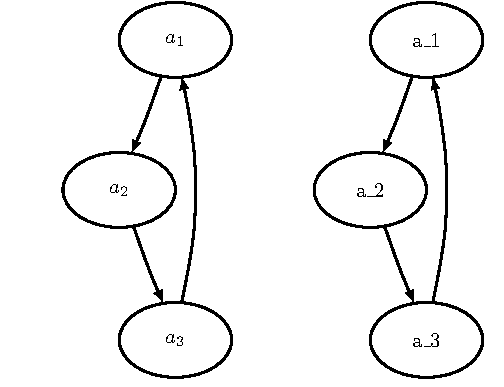
\includegraphics{pdf/ex1comb}
\end{figure}

Example of using \texttt{texlbl}:
\begin{quote}{\ttfamily \raggedright \noindent
digraph~G~{\{}~\\
~~~~a{\_}1~{[}texlbl="{\$}{\textbackslash}frac{\{}{\textbackslash}gamma{\}}{\{}x{\textasciicircum}2{\}}{\$}"{]};~\\
~~~~a{\_}1->~a{\_}2~->~a{\_}3~->~a{\_}1;~\\
{\}}
}\end{quote}
\begin{figure}[H]
\centering

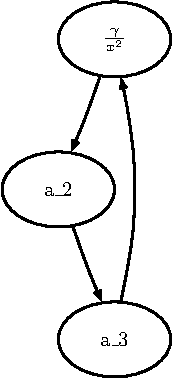
\includegraphics{pdf/ex2}
\end{figure}

Example of using the \texttt{texmode} attribute:
\begin{quote}{\ttfamily \raggedright \noindent
digraph~G~{\{}~\\
~~~~a{\_}1~{[}texlbl="{\$}{\textbackslash}frac{\{}{\textbackslash}gamma{\}}{\{}2x{\textasciicircum}2+y{\textasciicircum}3{\}}{\$}"{]};~\\
~~~~a{\_}1~->~a{\_}2~->~a{\_}3~->~a{\_}1~\\
~~~~node~{[}texmode="math"{]};~\\
~~~~a{\_}1~->~b{\_}1~->~b{\_}2~->~a{\_}3;~\\
~~~~b{\_}1~{[}label="{\textbackslash}{\textbackslash}frac{\{}{\textbackslash}{\textbackslash}gamma{\}}{\{}x{\textasciicircum}2{\}}"{]};~\\
~~~~node~{[}texmode="verbatim"{]}~\\
~~~~b{\_}4~{[}label="{\textbackslash}{\textbackslash}beta"{]}~\\
~~~~a{\_}3~->~b{\_}4~->~a{\_}1;~\\
{\}}
}\end{quote}
\begin{figure}[H]
\centering

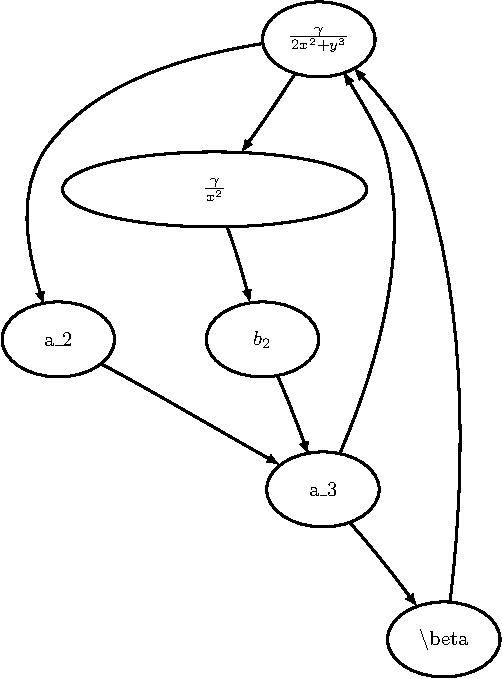
\includegraphics{pdf/texmode}
\end{figure}

The above example shows two important things:
\begin{itemize}
\item {} 
The backslash \texttt{{\textbackslash}} character needs to be written as \texttt{{\textbackslash}{\textbackslash}} in the \texttt{label} attribute.

\item {} 
Using LaTeX markup in the \texttt{label} attribute gives oversized nodes. A workaround  is to use the \texttt{texlbl} attribute, and manually pad the \texttt{label} attribute to an appropriate length. A much better solution is to use the \texttt{-{}-preproc} option.

\end{itemize}

Preprocessing the above graph with:
\begin{quote}{\ttfamily \raggedright \noindent
{\$}~dot2tex~-{}-preproc~ex4.dot~|~dot2tex~>~ex4.tex
}\end{quote}

gives correctly sized nodes:
\begin{figure}[H]
\centering

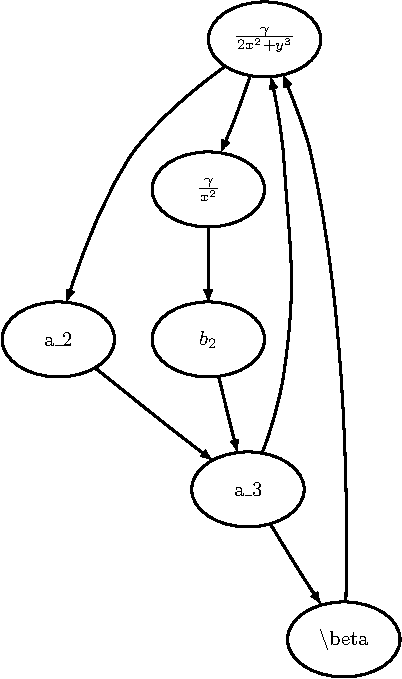
\includegraphics{pdf/texmodeb}
\end{figure}

Read more about preprocessing in the \href{\#preprocessing-graphs}{Preprocessing graphs} section.


%___________________________________________________________________________

\hypertarget{vertical-label-alignment}{}
\pdfbookmark[1]{Vertical label alignment}{vertical-label-alignment}
\subsection*{Vertical label alignment}
\label{vertical-label-alignment}

Dot2tex relies on the xdot format for drawing nodes and placing node labels. The fonts that Graphviz and LaTeX use are different, so using the label coordinates from Graphviz does not always give good results. Dot2tex's default behavior is to place node labels in the middle of the node. However, you can change this behavior by setting the \texttt{valignmode} option to \texttt{dot}. Labels will then be placed using the coordinates supplied by Graphviz.

Here is an example graph where it is necessary to use the \texttt{valignmode} option:
\begin{quote}{\ttfamily \raggedright \noindent
digraph~G~{\{}~\\
~~~~node0~{[}label="{\{}left|right{\}}",~shape=record{]};~\\
~~~~node1~{[}shape=rectangle,~label="node~1"{]};~\\
~~~~node0~->~node1;~\\
~~~~rankdir=LR;~\\
{\}}
}\end{quote}

For record nodes dot2tex has to use Graphviz coordinates. This is shown in the following figure rendered with:
\begin{quote}{\ttfamily \raggedright \noindent
{\$}~dot2tex~valign.dot
}\end{quote}
\begin{figure}[H]
\centering

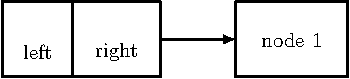
\includegraphics{pdf/valignmode0}
\end{figure}

To get the same vertical alignment for both nodes, you can use:
\begin{quote}{\ttfamily \raggedright \noindent
{\$}~dot2tex~-{}-valignmode=dot~valign.dot
}\end{quote}
\begin{figure}[H]
\centering

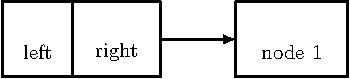
\includegraphics{pdf/valignmode1}
\end{figure}

Now the labels are aligned, but the labels are still placed too low. The reason for this is that both PSTricks and PGF by default centers text vertically on the current coordinate. The alignment point should in this case be set to the baseline. For PGF/TikZ you can use the \texttt{-{}-graphstyle} option like this:
\begin{quote}{\ttfamily \raggedright \noindent
{\$}~dot2tex~-{}-valignmode=dot~-{}-graphstyle="anchor=base"~valign.dot
}\end{quote}

PSTricks users have to use the \texttt{-{}-alingstr} option:
\begin{quote}{\ttfamily \raggedright \noindent
{\$}~dot2tex~-{}-valignmode=dot~-{}-alignstr=B~valign.dot
}\end{quote}
\begin{figure}[H]
\centering

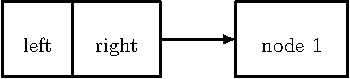
\includegraphics{pdf/valignmode2}
\end{figure}

The result is better, but to get even better alignment you have to change the node font size. Graphviz' default font size is 14pt, which is larger than the typical 10pt or 11pt used in LaTeX documents. By changing the node font size to 10pt we can trick Graphviz to give us a better alignment:
\begin{quote}{\ttfamily \raggedright \noindent
digraph~G~{\{}~\\
~~~~node~{[}fontsize=10{]};~\\
~~~~node0~{[}label="{\{}left|right{\}}",~shape=record{]};~\\
~~~~node1~{[}shape=rectangle,~label="node~1"{]};~\\
~~~~node0~->~node1;~\\
~~~~rankdir=LR;~\\
{\}}
}\end{quote}
\begin{figure}[H]
\centering

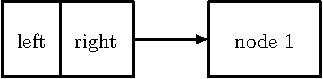
\includegraphics{pdf/valignmode3}
\end{figure}


%___________________________________________________________________________

\hypertarget{preprocessing-graphs}{}
\pdfbookmark[0]{Preprocessing graphs}{preprocessing-graphs}
\section*{Preprocessing graphs}
\label{preprocessing-graphs}

A problem with using LaTeX for typesetting node and edge labels, is that Graphviz does not know the sizes of the resulting labels. To circumvent this problem, you can use the \texttt{-{}-preproc} or \texttt{-{}-autosize} option. The following will then happen:
\newcounter{listcnt0}
\begin{list}{\arabic{listcnt0}.}
{
\usecounter{listcnt0}
\setlength{\rightmargin}{\leftmargin}
}
\item {} 
Node and edge labels are extracted and the corresponding LaTeX markup is saved to a temporary file.

\item {} 
The file is typeset with LaTeX and information about sizes is extracted using the \href{http://www.ctan.org/tex-archive/help/Catalogue/entries/preview.html}{preview} package.

\item {} 
A new dot file is created where node and edge label sizes are set using the dot language's \texttt{width} and \texttt{height} attributes.

\item {} 
The generated graph can now be processed using Graphviz and dot2tex. Label sizes will now correspond with the output from LaTeX.

\end{list}

Widths and heights of nodes are handled the in same way as Graphviz does it. The \texttt{width} and \texttt{height} attributes set the minimum size of the node. If label size + margins is larger that the minimum size, the node size will grow accordingly. Default values are width=0.75in and height=0.5in.

Node margins are set using the \href{http://graphviz.org/doc/info/attrs.html\#d:margin}{margin} attribute. This also works for edge labels. \texttt{margin==value} sets both the horizontal and vertical margin to \texttt{value}, \texttt{margin=="hvalue,vvalue"} sets the horizontal and vertical margins respectively.
\begin{center}\begin{sffamily}
\fbox{\parbox{\admonitionwidth}{
\textbf{\large Note}
\vspace{2mm}

All sizes are given in inches.
}}
\end{sffamily}
\end{center}

If you do not want a minimum node size, you can use the '-{}-nominsize' option. Dot2tex will then use size of label + margins as node size.

Nodes with \texttt{fixedsize=True} attributes are not processed.

Limitations:
\begin{itemize}
\item {} 
Does not work for HTML-labels

\item {} 
Does not work for record-based nodes

\end{itemize}


%___________________________________________________________________________

\hypertarget{examples}{}
\pdfbookmark[1]{Examples}{examples}
\subsection*{Examples}
\label{examples}

Consider the following graph:
\begin{quote}{\ttfamily \raggedright \noindent
digraph~G~{\{}~\\
~~~~node~{[}shape=circle{]};~\\
~~~~a{\_}1~{[}texlbl="{\$}x{\textasciicircum}2+{\textbackslash}frac{\{}{\textbackslash}sin~y{\}}{\{}y{\textasciicircum}2+{\textbackslash}cos~{\textbackslash}beta{\}}+{\textbackslash}gamma{\_}3{\$}"{]};~\\
~~~~a{\_}1~->~a{\_}2~{[}label="~",~texlbl="{\$}x{\_}1+x{\_}3{\textasciicircum}2+z+c+v{\textasciitilde}{\textasciitilde}{\$}"{]};~\\
~~~~a{\_}2~->~a{\_}1;~\\
{\}}
}\end{quote}

Rendered with:
\begin{quote}{\ttfamily \raggedright \noindent
{\$}~dot2tex~-tmath~example.dot~>~example.tex
}\end{quote}

the graph will look like this:
\begin{figure}[H]
\centering

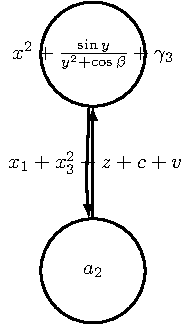
\includegraphics{pdf/preproc1a}
\end{figure}

You could improve the result by adding a longer \texttt{label} attribute or setting a fixed width. A better solution is to preprocess the graph like this:
\begin{quote}{\ttfamily \raggedright \noindent
{\$}~dot2tex~-tmath~-{}-preproc~example.dot~>~exampletmp.dot~\\
{\$}~dot2tex~exampletmp.dot~>~example.tex
}\end{quote}

You can also chain the commands:
\begin{quote}{\ttfamily \raggedright \noindent
{\$}~dot2tex~-tmath~-{}-preproc~example.dot~|~dot2tex~>~example.tex
}\end{quote}

A shorter alternative is:
\begin{quote}{\ttfamily \raggedright \noindent
{\$}~dot2tex~-tmath~-{}-autosize~example.dot~>~example.tex
}\end{quote}

The resulting graph now has correctly sized nodes and edge labels:
\begin{figure}[H]
\centering

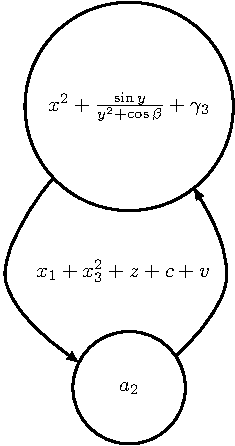
\includegraphics{pdf/preproc1b}
\end{figure}

Modifying node sizes using the \texttt{widht/height} and \texttt{margin} attributes can be a bit counterintuitive. A few examples will hopefully make it clearer:
\begin{quote}{\ttfamily \raggedright \noindent
digraph~G~{\{}~\\
~~~~node~{[}shape=rectangle{]};~\\
~~~~a{\_}1~{[}margin="0"{]};~\\
~~~~a{\_}2~{[}margin="0.7,0.4"{]};~\\
~~~~a{\_}3~{[}width="2",height="1"{]};~\\
~~~~a{\_}1->~a{\_}2~->~a{\_}3~->~a{\_}1;~\\
{\}}
}\end{quote}

Processing the graph with:
\begin{quote}{\ttfamily \raggedright \noindent
{\$}~dot2tex~-tmath~-{}-preproc~example.dot~|~dot2tex~>~example.tex
}\end{quote}

gives
\begin{figure}[H]
\centering

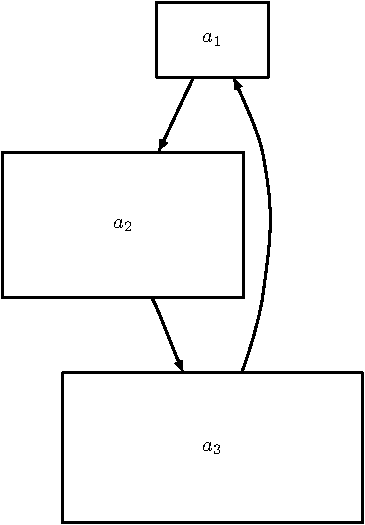
\includegraphics{pdf/nodewidth1}
\end{figure}

Setting the margin of \texttt{a{\_}1} to 0 has no effect because of the minimum node width. Processing the graph with:
\begin{quote}{\ttfamily \raggedright \noindent
{\$}~dot2tex~-tmath~-{}-preproc~-{}-nominsize~example.dot~|~dot2tex~>~example.tex
}\end{quote}

gives a different graph, where only label widths and margins affect the node sizes:
\begin{figure}[H]
\centering

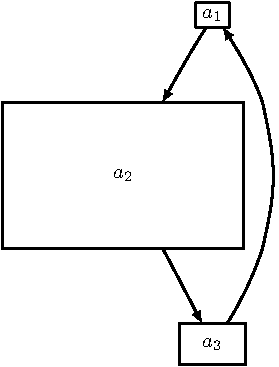
\includegraphics{pdf/nodewidth2}
\end{figure}


%___________________________________________________________________________

\hypertarget{customizing-the-output}{}
\pdfbookmark[0]{Customizing the output}{customizing-the-output}
\section*{Customizing the output}
\label{customizing-the-output}

Dot2tex offers a few ways of modifying the generated output.


%___________________________________________________________________________

\hypertarget{using-styles}{}
\pdfbookmark[1]{Using styles}{using-styles}
\subsection*{Using styles}
\label{using-styles}

The dot language defines the \texttt{style} attribute that can be used to modify the appearance of graphs, nodes, and edges. The \texttt{style} attribute is passed to the rendering backend, and is a powerful and flexible way of customizing the look and feel of your graphs. Using styles requires detailed knowledge of the output format.

The following example shows how interesting visual results can be achieved with the PGF/TikZ output format. The styles are PGF/TikZ specific. See the user guide for details:
\begin{quote}{\ttfamily \raggedright \noindent
graph~G~{\{}~\\
~~~~node~{[}shape=circle,~fixedsize=True,~width="0.2",~\\
~~~~~~~~~~style="ball~color~=green",~label="{}"{]};~\\
~~~~edge~{[}style="snake=zigzag,~green"{]};~\\
~~~~a{\_}1~-{}-~c~-{}-~a{\_}2;~\\
~~~~c~{[}style="ball~color=black"{]};~\\
~~~~edge~{[}style="snake=snake,~blue"{]};~\\
~~~~node~{[}style="ball~color~=~red",~label="{}"{]};~\\
~~~~a{\_}3~-{}-~c~-{}-~a{\_}4~-{}-a{\_}3;~\\
{\}}
}\end{quote}

The \texttt{snake} styles only work on straight lines. We therefore have to use the \texttt{-s} option. \texttt{fdp} is used to lay out the graph:
\begin{quote}{\ttfamily \raggedright \noindent
{\$}~fdp~-TXdot~ball.dot~|~dot2tex~-fpgf~-s~>~balls.tex
}\end{quote}

The resulting graph is shown below.
\begin{figure}[H]
\centering

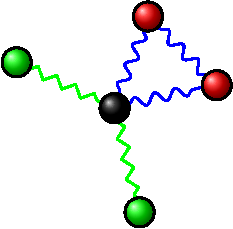
\includegraphics{pdf/balls}
\end{figure}
\begin{center}\begin{sffamily}
\fbox{\parbox{\admonitionwidth}{
\textbf{\large Note}
\vspace{2mm}

Use the straight edge option \texttt{-s} to force the use of straight lines. Otherwise curves will be used to draw even straight lines.
}}
\end{sffamily}
\end{center}


%___________________________________________________________________________

\hypertarget{changing-arrow-types}{}
\pdfbookmark[2]{Changing arrow types}{changing-arrow-types}
\subsubsection*{Changing arrow types}
\label{changing-arrow-types}

The style attribute can be used to change arrow types. A PGF/TikZ example:
\begin{quote}{\ttfamily \raggedright \noindent
digraph~G~{\{}~\\
~~~~graph~{[}mindist=0.5{]};~\\
~~~~node~{[}fixedsize=true,~shape=circle,~width=0.4,~style="fill=green!20"{]};~\\
~~~~c~->~n{\_}1~{[}style="-stealth"{]};~\\
~~~~c~->~n{\_}2~{[}style="-to"{]};~\\
~~~~c~->~n{\_}3~{[}style="-latex"{]};~\\
~~~~c~->~n{\_}4~{[}style="-diamond"{]};~\\
~~~~c~->~n{\_}5~{[}style="-o"{]};~\\
~~~~c~->~n{\_}6~{[}style="{\{}-{]}{\}}"{]};~\\
~~~~c~->~n{\_}7~{[}style="-triangle~90"{]};~\\
~~~~c~->~n{\_}8~{[}style="-hooks"{]};~\\
~~~~c~->~n{\_}9~{[}style="->{}>"{]};~\\
~~~~c~{[}style="fill=red!80"{]};~\\
{\}}
}\end{quote}

Rendered with:
\begin{quote}{\ttfamily \raggedright \noindent
{\$}~circo~-Txdot~pgfarrows.dot~|~dot2tex~-tmath~>~pgfarrows.tex
}\end{quote}
\begin{figure}[H]
\centering

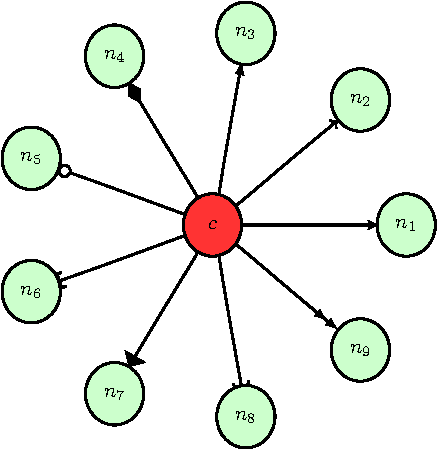
\includegraphics{pdf/pgfarrows}
\end{figure}

You can also set the default arrow style by using the \texttt{-{}-graphstyle} option or \texttt{d2tgraphstyle} attribute:
\begin{quote}{\ttfamily \raggedright \noindent
{\$}~dot2tex~-tmath~-{}-graphstyle=">=diamond"~ex1.dot~>~ex1gstyle.tex
}\end{quote}
\begin{figure}[H]
\centering

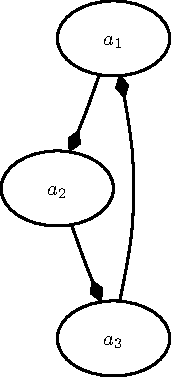
\includegraphics{pdf/ex1gstyle}
\end{figure}

A PSTricks example:
\begin{quote}{\ttfamily \raggedright \noindent
digraph~G~{\{}~\\
~~~~d2tdocpreamble="{\textbackslash}usepackage{\{}pstricks-add{\}}";~\\
~~~~graph~{[}mindist=0.5{]};~\\
~~~~node~{[}texmode="math",~fixedsize=true,~shape=circle,~width=0.4{]};~\\
~~~~c~->~n{\_}1~{[}style="arrows=->"{]};~\\
~~~~c~->~n{\_}2~{[}style="arrows=->{}>"{]};~\\
~~~~c~->~n{\_}3~{[}style="arrows=-<"{]};~\\
~~~~c~->~n{\_}4~{[}style="arrows=-*"{]};~\\
~~~~c~->~n{\_}5~{[}style="arrows=-{\{}{]}{\}}"{]};~\\
~~~~c~->~n{\_}6~{[}style="arrows=-o"{]};~\\
~~~~c~->~n{\_}7~{[}style="arrows=-H"{]};~\\
{\}}
}\end{quote}

Rendered with:
\begin{quote}{\ttfamily \raggedright \noindent
{\$}~circo~-Txdot~pstarrows.dot~|~dot2tex~-fpst~>~pstarrows.tex
}\end{quote}
\begin{figure}[H]
\centering

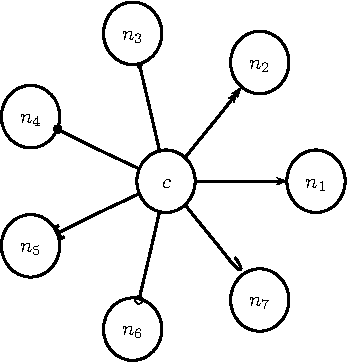
\includegraphics{pdf/pstarrows}
\end{figure}

The above example shows how the \texttt{d2tdocpreamble} attribute can be used to load additional LaTeX packages. You could also use the \texttt{`-{}-docpreamble} option:
\begin{quote}{\ttfamily \raggedright \noindent
{\$}~...~|~dot2tex~-fpst~-{}-docpreamble="{\textbackslash}usepackage{\{}pstricks-add{\}}"~...
}\end{quote}


%___________________________________________________________________________

\hypertarget{label-styles}{}
\pdfbookmark[2]{Label styles}{label-styles}
\subsubsection*{Label styles}
\label{label-styles}

Node, edge and graph labels can be styled using the special \texttt{lblstyle} attribute. However, this only works for the \texttt{pgf} and \texttt{tikz} output formats.

Labels are drawn using code like:
\begin{quote}{\ttfamily \raggedright \noindent
{\textbackslash}draw~(157bp,52bp)~node~{\{}label{\}};
}\end{quote}

When you specify a \texttt{lblstyle} attribute, the style will be given as a parameter to the node like this:
\begin{quote}{\ttfamily \raggedright \noindent
{\textbackslash}draw~(157bp,52bp)~node{[}lblstyle{]}~{\{}label{\}};
}\end{quote}

Example:
\begin{quote}{\ttfamily \raggedright \noindent
digraph~G~{\{}~\\
~~~~node~{[}shape=circle{]};~\\
~~~~a~->~b~{[}label="label",lblstyle="draw=red,cross~out"{]};~\\
~~~~b~->~c~{[}label="test",lblstyle="below=0.5cm,rotate=20,fill=blue!20"{]};~\\
~~~~a~{[}label="aa",lblstyle="blue"{]};~\\
~~~~b~{[}lblstyle="font={\textbackslash}Huge"{]};~\\
~~~~c~{[}label="ccc",~lblstyle="red,rotate=90"{]};~\\
~~~~label="Graph~label";~\\
~~~~lblstyle="draw,fill=red!20";~\\
~~~~rankdir=LR;~\\
{\}}
}\end{quote}
\begin{figure}[H]
\centering

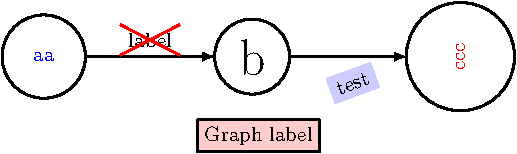
\includegraphics{pdf/lblstyle}
\end{figure}

See the PGF and TikZ documentation for more information about styles.
\begin{center}\begin{sffamily}
\fbox{\parbox{\admonitionwidth}{
\textbf{\large Note}
\vspace{2mm}

You can use the \texttt{exstyle} attribute in addition to \texttt{lblstyle}. The difference is that \texttt{exstyle} is ignored in preprocessing mode. Useful when using TikZ' \texttt{pin} and \texttt{label} options and you do not want them to influence the graph layout.
}}
\end{sffamily}
\end{center}


%___________________________________________________________________________

\hypertarget{node-and-edge-options}{}
\pdfbookmark[2]{Node and edge options}{node-and-edge-options}
\subsubsection*{Node and edge options}
\label{node-and-edge-options}

The \texttt{tikz} output format offers an additional way of customizing the output by using the \texttt{-{}-nodeoptions} and \texttt{-{}-edgeoptions} options, or the \texttt{d2tnodeoptions} and \texttt{d2tedgeoptions} graph attributes. The code for generating nodes and edges will then be wrapped in a \texttt{scope} environment like this:
\begin{quote}{\ttfamily \raggedright \noindent
...~\\
{\textbackslash}begin{\{}scope{\}}{[}nodeoptions{]}~\\
{\%}~code~for~drawing~nodes~\\
{\textbackslash}end{\{}scope{\}}~\\
{\textbackslash}begin{\{}scope{\}}{[}edgeoptions{]}~\\
{\%}~code~for~drawing~edges~\\
{\textbackslash}end{\{}scope{\}}~\\
...
}\end{quote}


%___________________________________________________________________________

\hypertarget{customizing-edges}{}
\pdfbookmark[0]{Customizing edges}{customizing-edges}
\section*{Customizing edges}
\label{customizing-edges}

The \texttt{tikz} and \texttt{pgf} output formats offers a few additional ways of customizing how edges are drawn and how edge edge labels are placed. These features are tightly integrated with TikZ and detailed knowledge of the output format is therefore necessary.


%___________________________________________________________________________

\hypertarget{tikz-edge-labels}{}
\pdfbookmark[1]{TikZ edge labels}{tikz-edge-labels}
\subsection*{TikZ edge labels}
\label{tikz-edge-labels}

With the \texttt{-{}-tikzedgelabel} option you can bypass the XDOT edge label placement and let PGF and TikZ do the job instead. This can be useful in some cases. However, this only works properly for straight edges and \texttt{to} paths.

Example:
\begin{quote}{\ttfamily \raggedright \noindent
graph~G~{\{}~\\
~~~~mindist~=~0.5;~\\
~~~~node~{[}shape="circle"{]};~\\
~~~~edge~{[}lblstyle="mystyle"{]};~\\
~~~~a~-{}-~b~{[}label="ab"{]};~\\
~~~~b~-{}-~c~{[}label="bc"{]};~\\
~~~~c~-{}-~a~{[}label="ca"{]};~\\
{\}}
}\end{quote}

Without the \texttt{-{}-tikzedgelabel} option the code for placing edges will look something like this:
\begin{quote}{\ttfamily \raggedright \noindent
{\%}~Edge:~a~-{}-~b~\\
{\textbackslash}draw~{[}{]}~(28bp,55bp)~-{}-~(28bp,75bp);~\\
{\textbackslash}draw~(40bp,65bp)~node{[}mystyle{]}~{\{}ab{\}};~\\
{\%}~Edge:~b~-{}-~c~\\
{\textbackslash}draw~{[}{]}~(51bp,88bp)~-{}-~(68bp,78bp);~\\
{\textbackslash}draw~(66bp,96bp)~node{[}mystyle{]}~{\{}bc{\}};~\\
{\%}~Edge:~c~-{}-~a~\\
{\textbackslash}draw~{[}{]}~(69bp,51bp)~-{}-~(52bp,41bp);~\\
{\textbackslash}draw~(53bp,57bp)~node{[}mystyle{]}~{\{}ca{\}};
}\end{quote}

With the \texttt{tikzedgelabels} option the output is simply:
\begin{quote}{\ttfamily \raggedright \noindent
{\textbackslash}draw~{[}{]}~(a)~-{}-~node{[}mystyle{]}~{\{}ab{\}}~(b);~\\
{\textbackslash}draw~{[}{]}~(b)~-{}-~node{[}mystyle{]}~{\{}bc{\}}~(c);~\\
{\textbackslash}draw~{[}{]}~(c)~-{}-~node{[}mystyle{]}~{\{}ca{\}}~(a);
}\end{quote}

The placement of the edge labels depends on the options passed to the edge label node (in this case \texttt{mystyle}), and the curve used to connect the nodes. Some examples of \texttt{mystyle} values are shown in the figure below. The leftmost graph is rendered without the \texttt{tikzedgelabels} option.
\begin{figure}[H]
\centering

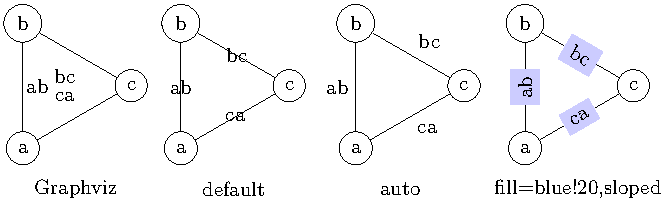
\includegraphics{pdf/tikzedgelabels}
\end{figure}

Limitations:
\begin{itemize}
\item {} 
Works best with straight edges and \texttt{to} paths

\item {} 
The \texttt{headlabel} and \texttt{taillabel} attributes are currently not affected by the \texttt{tikzedgelabels} option.

\end{itemize}


%___________________________________________________________________________

\hypertarget{to-paths}{}
\pdfbookmark[1]{To paths}{to-paths}
\subsection*{To paths}
\label{to-paths}

The \texttt{topath} edge attribute offers a way to override the edges drawn by Graphviz. When a \texttt{topath} attribute is encountered, dot2tex inserts a so called \texttt{to} path operation to connect the nodes. A number of predefined to paths are defined by TikZ, and you can create your own.

Example:
\begin{quote}{\ttfamily \raggedright \noindent
digraph~G~{\{}~\\
~~~~mindist~=~0.5;~\\
~~~~node~{[}shape="circle"{]};~\\
~~~~a~->~b~{[}topath="bend~right"{]};~\\
~~~~c~->~b~{[}topath="bend~left"{]};~\\
~~~~c~->~a~{[}topath="out=10,in=-90"{]};~\\
~~~~b~->~b~{[}topath="loop~above"{]};~\\
{\}}
}\end{quote}

Generating the graph with:
\begin{quote}{\ttfamily \raggedright \noindent
{\$}~circo~-Txdot~topaths1.dot~|~dot2tex~-ftikz~>~topaths1.tex
}\end{quote}

yields:
\begin{figure}[H]
\centering

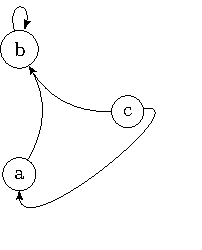
\includegraphics{pdf/topaths1}
\end{figure}

The generated edge drawing code is:
\begin{quote}{\ttfamily \raggedright \noindent
{\textbackslash}draw~{[}->{]}~(a)~to{[}bend~right{]}~(b);~\\
{\textbackslash}draw~{[}->{]}~(c)~to{[}bend~left{]}~(b);~\\
{\textbackslash}draw~{[}->{]}~(c)~to{[}out=10,in=-90{]}~(a);~\\
{\textbackslash}draw~{[}->{]}~(b)~to{[}loop~above{]}~(b);
}\end{quote}
\begin{center}\begin{sffamily}
\fbox{\parbox{\admonitionwidth}{
\textbf{\large Note}
\vspace{2mm}

To paths works best with layout tools that generate straight edges (neato, fdp, circo, twopi). The \texttt{topath} attribute overrides the edge routing done by Graphviz. You may therefore end up with overlapping edges.
}}
\end{sffamily}
\end{center}

Here is a larger example that uses the \texttt{automata} library:
\begin{quote}{\ttfamily \raggedright \noindent
digraph~G~{\{}~\\
~~~~d2tdocpreamble~=~"{\textbackslash}usetikzlibrary{\{}automata{\}}";~\\
~~~~d2tfigpreamble~=~"{\textbackslash}tikzstyle{\{}every~state{\}}=~{\textbackslash}~\\
~~~~{[}draw=blue!50,very~thick,fill=blue!20{]}";~\\
~~~~node~{[}style="state"{]};~\\
~~~~edge~{[}lblstyle="auto",topath="bend~left"{]};~\\
~~~~A~{[}style="state,~initial"{]};~\\
~~~~A~->~B~{[}label=2{]};~\\
~~~~A~->~D~{[}label=7{]};~\\
~~~~B~->~A~{[}label=1{]};~\\
~~~~B~->~B~{[}label=3,topath="loop~above"{]};~\\
~~~~B~->~C~{[}label=4{]};~\\
~~~~C~->~F~{[}label=5{]};~\\
~~~~F~->~B~{[}label=8{]};~\\
~~~~F~->~D~{[}label=7{]};~\\
~~~~D~->~E~{[}label=2{]};~\\
~~~~E~->~A~{[}label="1,6"{]};~\\
~~~~F~{[}style="state,accepting"{]};~\\
{\}}
}\end{quote}

Generated with:
\begin{quote}{\ttfamily \raggedright \noindent
neato~-Txdot~fsm1.dot~|~dot2tex~-ftikz~-{}-tikzedgelabels~-{}-styleonly
}\end{quote}
\begin{figure}[H]
\centering

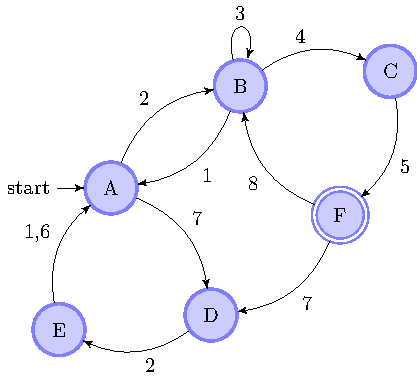
\includegraphics{pdf/fsm1}
\end{figure}


%___________________________________________________________________________

\hypertarget{color-support}{}
\pdfbookmark[0]{Color support}{color-support}
\section*{Color support}
\label{color-support}

All Graphviz \href{http://www.graphviz.org/doc/info/attrs.html\#k:color}{color formats} are supported, including the RGBA format. Transparency will however only work when using the PGF/TikZ output format.

Named colors are supported, but you have to ensure that the colors are defined in the resulting LaTeX file. The default PSTricks and PGF/TikZ templates load the \texttt{X11names} color scheme defined in the \href{http://www.ctan.org/tex-archive/help/Catalogue/entries/xcolor.html}{xcolor} package. Note that color names in the \href{http://www.ctan.org/tex-archive/help/Catalogue/entries/xcolor.html}{xcolor} package are case sensitive. This is not the case with Graphviz's \href{http://www.graphviz.org/doc/info/colors.html}{color names}. Use \href{http://en.wikipedia.org/wiki/CamelCase}{CamelCase}  names in your graphs to ensure compatibility with \href{http://www.ctan.org/tex-archive/help/Catalogue/entries/xcolor.html}{xcolor}.

For convenience, a color definition file \texttt{gcols.tex} is distributed with dot2tex. You can find it in the \texttt{examples} directory. This file defines most of Graphviz's named colors as lower case. Include this file in the preamble if you need it.


%___________________________________________________________________________

\hypertarget{templates}{}
\pdfbookmark[0]{Templates}{templates}
\section*{Templates}
\label{templates}

The output from dot2tex is a list of drawing commands. To render the graphics with LaTeX there's a need for some boiling plate code. This code can be customized using simple templates. If no template is specified with the \titlereference{-{}-template} option, a default template will be used.

The following template tags are available:
\begin{description}
\item[{\texttt{<{}<drawcommands>{}>}}] \leavevmode 
The actual list of drawing commands.

\item[{\texttt{<{}<figcode>{}>}}] \leavevmode 
Drawing commands wrapped in a figure environment. Note that several important style options are set in the figure environment.

\item[{\texttt{<{}<bbox>{}>}}] \leavevmode 
Bounding box. Example: \texttt{(0bp,0bp)(100bp,100bp)}
The individual parts of the bounding box are available with the tags:
\begin{itemize}
\item {} 
\texttt{<{}<bbox.x0>{}>}

\item {} 
\texttt{<{}<bbox.y0>{}>}

\item {} 
\texttt{<{}<bbox.x1>{}>}

\item {} 
\texttt{<{}<bbox.y1>{}>}

\end{itemize}

Note that the bounding box parts are given without any units.

\item[{\texttt{<{}<textencoding>{}>}}] \leavevmode 
The text encoding used for the output file. Current values are:
- \texttt{utf8}
- \texttt{latin1}

\item[{\texttt{<{}<docpreamble>{}>}}] \leavevmode 
Document preamble. The content of this tag is set by the \texttt{-{}-docpreamble} option or \texttt{d2tdocpreamble} graph attribute. Useful for including packages and such.

\item[{\texttt{<{}<figpreamble>{}>}}] \leavevmode 
Figure preamble. The content of this tag is set by the \texttt{-{}-figpreamble} option or \texttt{d2tfigpreamble} graph attribute. Useful for setting font sizes and such.

\item[{\texttt{<{}<preproccode>{}>}}] \leavevmode 
Code generated for preprocessing labels.

\end{description}

Three different templates are used by dot2tex for the preprocessing mode, output mode and figure only mode respectively. The following template tags make it possible to use the same template file for all modes.
\begin{description}
\item[{\texttt{<{}<startoutputsection>{}>} and \texttt{<{}<endoutputsection>{}>}}] \leavevmode 
Code between these tags is ignored in preprocessing mode.

\item[{\texttt{<{}<startpreprocsection>{}>} and \texttt{<{}<endpreprocsection>{}>}}] \leavevmode 
Code between these tags is ignored in output mode.

\item[{\texttt{<{}<startfigonlysection>{}>} and \texttt{<{}<endfigonlysection>{}>}}] \leavevmode 
Code between these tags is used as a template when using the \texttt{-{}-figonly} option. Ignored in preprocessing and output mode.

\end{description}
\begin{center}\begin{sffamily}
\fbox{\parbox{\admonitionwidth}{
\textbf{\large Note}
\vspace{2mm}

Tags that have no value are replaced with an empty string. Insert a \texttt{{\%}} character after a template tag to avoid unwanted line breaks.
}}
\end{sffamily}
\end{center}


%___________________________________________________________________________

\hypertarget{default-pgf-tikz-template}{}
\pdfbookmark[1]{Default PGF/TikZ template}{default-pgf-tikz-template}
\subsection*{Default PGF/TikZ template}
\label{default-pgf-tikz-template}
\begin{quote}{\ttfamily \raggedright \noindent
{\textbackslash}documentclass{\{}article{\}}~\\
{\textbackslash}usepackage{[}x11names,~rgb{]}{\{}xcolor{\}}~\\
{\textbackslash}usepackage{[}<{}<textencoding>{}>{]}{\{}inputenc{\}}~\\
{\textbackslash}usepackage{\{}tikz{\}}~\\
{\textbackslash}usetikzlibrary{\{}snakes,arrows,shapes{\}}~\\
{\textbackslash}usepackage{\{}amsmath{\}}~\\
<{}<startpreprocsection>{}>{\%}~\\
{\textbackslash}usepackage{[}active,auctex{]}{\{}preview{\}}~\\
<{}<endpreprocsection>{}>{\%}~\\
<{}<gvcols>{}>{\%}~\\
<{}<cropcode>{}>{\%}~\\
<{}<docpreamble>{}>{\%}~\\
~\\
{\textbackslash}begin{\{}document{\}}~\\
{\textbackslash}pagestyle{\{}empty{\}}~\\
{\%}~\\
<{}<startpreprocsection>{}>{\%}~\\
<{}<preproccode>{}>~\\
<{}<endpreprocsection>{}>{\%}~\\
{\%}~\\
<{}<startoutputsection>{}>~\\
{\textbackslash}enlargethispage{\{}100cm{\}}~\\
{\%}~Start~of~code~\\
{\%}~{\textbackslash}begin{\{}tikzpicture{\}}{[}anchor=mid,>=latex',join=bevel,<{}<graphstyle>{}>{]}~\\
{\textbackslash}begin{\{}tikzpicture{\}}{[}>=latex',join=bevel,<{}<graphstyle>{}>{]}~\\
{\textbackslash}pgfsetlinewidth{\{}1bp{\}}~\\
<{}<figpreamble>{}>{\%}~\\
<{}<drawcommands>{}>~\\
<{}<figpostamble>{}>{\%}~\\
{\textbackslash}end{\{}tikzpicture{\}}~\\
{\%}~End~of~code~\\
<{}<endoutputsection>{}>~\\
{\%}~\\
{\textbackslash}end{\{}document{\}}~\\
{\%}~\\
<{}<startfigonlysection>{}>~\\
{\textbackslash}begin{\{}tikzpicture{\}}{[}>=latex,join=bevel,<{}<graphstyle>{}>{]}~\\
{\textbackslash}pgfsetlinewidth{\{}1bp{\}}~\\
<{}<figpreamble>{}>{\%}~\\
<{}<drawcommands>{}>~\\
<{}<figpostamble>{}>{\%}~\\
{\textbackslash}end{\{}tikzpicture{\}}~\\
<{}<endfigonlysection>{}>
}\end{quote}

The \texttt{<{}<cropcode>{}>} template tag is available when the \texttt{-{}-preview} option is used. The contents will then be:
\begin{quote}{\ttfamily \raggedright \noindent
{\textbackslash}usepackage{[}active,tightpage{]}{\{}preview{\}}~\\
{\textbackslash}PreviewEnvironment{\{}tikzpicture{\}}~\\
{\textbackslash}setlength{\textbackslash}PreviewBorder{\{}<{}<margin>{}>{\}}
}\end{quote}


%___________________________________________________________________________

\hypertarget{default-pstricks-template}{}
\pdfbookmark[1]{Default pstricks template}{default-pstricks-template}
\subsection*{Default pstricks template}
\label{default-pstricks-template}
\begin{quote}{\ttfamily \raggedright \noindent
{\textbackslash}documentclass{\{}article{\}}~\\
{\%}~<{}<bbox>{}>~\\
{\textbackslash}usepackage{[}x11names{]}{\{}xcolor{\}}~\\
{\textbackslash}usepackage{[}<{}<textencoding>{}>{]}{\{}inputenc{\}}~\\
{\textbackslash}usepackage{\{}graphicx{\}}~\\
{\textbackslash}usepackage{\{}pstricks{\}}~\\
{\textbackslash}usepackage{\{}amsmath{\}}~\\
<{}<startpreprocsection>{}>{\%}~\\
{\textbackslash}usepackage{[}active,auctex{]}{\{}preview{\}}~\\
<{}<endpreprocsection>{}>{\%}~\\
<{}<gvcols>{}>{\%}~\\
<{}<docpreamble>{}>{\%}~\\
~\\
~\\
{\textbackslash}begin{\{}document{\}}~\\
{\textbackslash}pagestyle{\{}empty{\}}~\\
<{}<startpreprocsection>{}>{\%}~\\
<{}<preproccode>{}>{\%}~\\
<{}<endpreprocsection>{}>{\%}~\\
<{}<startoutputsection>{}>{\%}~\\
{\textbackslash}enlargethispage{\{}100cm{\}}~\\
~\\
{\%}~Start~of~code~\\
{\textbackslash}begin{\{}pspicture{\}}{[}linewidth=1bp<{}<graphstyle>{}>{]}<{}<bbox>{}>~\\
{\textbackslash}pstVerb{\{}2~setlinejoin{\}}~{\%}~set~line~join~style~to~'mitre'~\\
<{}<figpreamble>{}>{\%}~\\
<{}<drawcommands>{}>~\\
<{}<figpostamble>{}>{\%}~\\
{\textbackslash}end{\{}pspicture{\}}~\\
{\%}~End~of~code~\\
<{}<endoutputsection>{}>{\%}~\\
{\textbackslash}end{\{}document{\}}~\\
{\%}~\\
<{}<startfigonlysection>{}>~\\
{\textbackslash}begin{\{}pspicture{\}}{[}linewidth=1bp<{}<graphstyle>{}>{]}<{}<bbox>{}>~\\
{\textbackslash}pstVerb{\{}2~setlinejoin{\}}~{\%}~set~line~join~style~to~'mitre'~\\
<{}<figpreamble>{}>{\%}~\\
<{}<drawcommands>{}>~\\
<{}<figpostamble>{}>{\%}~\\
{\textbackslash}end{\{}pspicture{\}}~\\
<{}<endfigonlysection>{}>
}\end{quote}


%___________________________________________________________________________

\hypertarget{special-attributes}{}
\pdfbookmark[0]{Special attributes}{special-attributes}
\section*{Special attributes}
\label{special-attributes}

Dot2tex defines several special graph, node and edge attributes. Most of them are not part of the DOT language.
\begin{description}
\item[{\texttt{texmode}}] \leavevmode 
Changes locally how \href{\#labels}{labels} are interpreted.

\item[{\texttt{texlbl}}] \leavevmode 
Overrides the current node or edge label.

\item[{\texttt{d2tdocpreamble}}] \leavevmode 
Sets the \texttt{<{}<docpreamble>{}>} tag.

\item[{\texttt{d2tfigpreamble}}] \leavevmode 
Sets the \texttt{<{}<figpreamble>{}>} tag.

\item[{\texttt{d2tfigpostamble}}] \leavevmode 
Sets the \texttt{<{}<figpostable>{}>} tag.

\item[{\texttt{d2tgraphstyle}}] \leavevmode 
Sets the \texttt{<{}<graphstyle>{}>} tag.

\item[{\texttt{d2ttikzedgelabels}}] \leavevmode 
Sets the \texttt{-{}-tikzedgelabels} option.

\item[{\texttt{d2tnodeoptions}}] \leavevmode 
Sets the \texttt{-{}-nodeoptions} option.

\item[{\texttt{d2tedgeoptions}}] \leavevmode 
Sets the \texttt{-{}-edgeoptions} option.

\item[{\texttt{style}}] \leavevmode 
Used to pass styles to the backend. Styles are output format specific, with the exception of the styles defined by the DOT language.

\item[{\texttt{lblstyle}}] \leavevmode 
Used to set styles for drawing graph, node and edge labels. Only works for the \texttt{pgf} and \texttt{tikz} output formats.

\item[{\texttt{exstyle}}] \leavevmode 
The same as \texttt{lblstyle}, except that \texttt{exstyle} is ignored in preprocessing mode.

\item[{\texttt{topath}}] \leavevmode 
Used to set a \texttt{to} path operation for connecting nodes. Only works for the \texttt{tikz} output format.

\item[{\texttt{d2talignstr}}] \leavevmode 
Used to pass a default alignment string to the PSTricks \texttt{{\textbackslash}rput} command:
\begin{quote}{\ttfamily \raggedright \noindent
{\textbackslash}rput{[}d2talignstr{]}~...
}\end{quote}

\item[{\texttt{d2toptions}}] \leavevmode 
Allows you to pass options to dot2tex in the same format as from the command line. The \texttt{d2toptions} value is parsed in the same way as ordinary command line options.

\end{description}


%___________________________________________________________________________

\hypertarget{issues-and-limitations}{}
\pdfbookmark[0]{Issues and limitations}{issues-and-limitations}
\section*{Issues and limitations}
\label{issues-and-limitations}

The purpose of dot2tex is to give graphs a more LaTeX friendly look, not to create exact duplicates. However, the program does a descent duplication job when it comes to drawing nodes and edges, but it does not try to duplicate label and annotation formatting.

A list of known limitations:
\begin{itemize}
\item {} 
Parallel edges are only supported in the \texttt{duplicate} mode.

\item {} 
Background color of page is currently not set.

\item {} 
The \texttt{fontcolor} attribute is not supported yet.

\item {} 
The \texttt{setlinewidth(.)} attribute is not supported yet.

\item {} 
Pydot/Pyparsing have some problems with the HTML syntax.

\item {} 
Pydot/Pyparsing sometimes choke on valid dot files. If this happen you could try to feed xdot data directly to dot2tex like this:
\begin{quote}{\ttfamily \raggedright \noindent
{\$}~dot~-Txdot~example.dot~|~dot2tex~-o~example.tex
}\end{quote}

\end{itemize}


%___________________________________________________________________________

\hypertarget{text-encoding}{}
\pdfbookmark[1]{Text encoding}{text-encoding}
\subsection*{Text encoding}
\label{text-encoding}

Graphviz's default text encoding is \texttt{utf8}. The \texttt{latin1} encoding can also be used. Utf8 is an unicode encoding and can in theory handle any international characters. However, LaTeX's unicode support is somewhat limited.


%___________________________________________________________________________

\hypertarget{tips-and-tricks}{}
\pdfbookmark[0]{Tips and tricks}{tips-and-tricks}
\section*{Tips and tricks}
\label{tips-and-tricks}


%___________________________________________________________________________

\hypertarget{fonts}{}
\pdfbookmark[1]{Fonts}{fonts}
\subsection*{Fonts}
\label{fonts}

No font information in the DOT file is preserved by dot2tex. However, there are several ways of  modifying the generated LaTeX code to achieve some control of fonts and font sizes.
\begin{itemize}
\item {} 
Modifying the templates.

\item {} 
Using the \texttt{d2tdocpreamble} and \texttt{d2tfigpreamble} attributes or command line options.

\item {} 
Using the \texttt{lblstyle} attribute.

\end{itemize}

To increase the font size you can for instance insert a \texttt{{\textbackslash}Huge} command in the figure preamble:
\begin{quote}{\ttfamily \raggedright \noindent
{\$}~dot2tex~-tmath~-{}-figpreamble="{\textbackslash}Huge"~ex1.dot~>~ex1huge.tex
}\end{quote}
\begin{figure}[H]
\centering

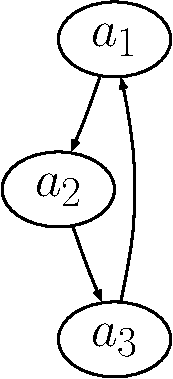
\includegraphics{pdf/ex1huge}
\end{figure}


%___________________________________________________________________________

\hypertarget{debugging}{}
\pdfbookmark[1]{Debugging}{debugging}
\subsection*{Debugging}
\label{debugging}

When making your own templates it is easy to make mistakes, and LaTeX markup in graphs may fail to compile. To make it easier to find errors, invoke dot2tex with the \texttt{-{}-debug} option:
\begin{quote}{\ttfamily \raggedright \noindent
{\$}~dot2tex~-{}-preproc~-{}-debug~test.dot
}\end{quote}

A dot2tex.log file will then be generated with detailed information. In the log file you will find the generated LaTeX code, as well as well as the compilation log.


%___________________________________________________________________________

\hypertarget{be-consistent}{}
\pdfbookmark[1]{Be consistent}{be-consistent}
\subsection*{Be consistent}
\label{be-consistent}

Be aware of differences between the template you use for preprocessing and code used to generate final output. This is especially important if you use the \texttt{-{}-figonly} option and include the code in a master document. If a 10pt font is used during preprocessing, the result may not be optimal if a 12pt font is used in the final output.

Example. A graph is generated with:
\begin{quote}{\ttfamily \raggedright \noindent
{\$}~dot2tex~-{}-preproc~-tmath~-{}-nominsize~ex1.dot~>~ex1tmp.dot
}\end{quote}

Running through dot2tex again with:
\begin{quote}{\ttfamily \raggedright \noindent
{\$}~dot2tex~-{}-figpreamble="{\textbackslash}Huge"~ex1tmp.dot~>~ex1huge.tex
}\end{quote}

gives labels that do not fit properly inside the nodes.
\begin{figure}[H]
\centering

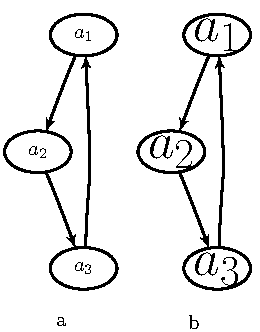
\includegraphics{pdf/consistent}
\end{figure}


%___________________________________________________________________________

\hypertarget{postprocessing}{}
\pdfbookmark[1]{Postprocessing}{postprocessing}
\subsection*{Postprocessing}
\label{postprocessing}

The output from Graphviz and dot2tex is not perfect. Manual adjustments are sometimes necessary to get the right results for use in a publication. For final and cosmetic adjustments, it is often easier to edit the generated code than to hack the dot source. This is especially true when using the \texttt{tikz} output format.


%___________________________________________________________________________

\hypertarget{use-the-special-graph-attributes}{}
\pdfbookmark[1]{Use the special graph attributes}{use-the-special-graph-attributes}
\subsection*{Use the special graph attributes}
\label{use-the-special-graph-attributes}

Dot2tex has many options for customizing the output. Sometimes is is impractical or boring to type the various options at the command line each time you want to create the graph. To avoid this, you can use the special graph attributes. The \texttt{d2toptions} attribute is handy because it is interpreted as command line options.

So instead of typing:
\begin{quote}{\ttfamily \raggedright \noindent
{\$}~dot2tex~-tikz~-tmath~-{}-tikzedgelabels~ex1.dot
}\end{quote}

each time, use \texttt{d2toptions} like this:
\begin{quote}{\ttfamily \raggedright \noindent
digraph~G~{\{}~\\
~~~~d2toptions~="-tikz~-tmath~-{}-tikzedgelabels";~\\
~~~~...~\\
{\}}
}\end{quote}


%___________________________________________________________________________

\hypertarget{use-the-tikz-output-format-for-maximum-flexibility}{}
\pdfbookmark[1]{Use the tikz output format for maximum flexibility}{use-the-tikz-output-format-for-maximum-flexibility}
\subsection*{Use the tikz output format for maximum flexibility}
\label{use-the-tikz-output-format-for-maximum-flexibility}

The difference between the \texttt{pgf} and \texttt{tikz} output formats is best shown with an example. Consider the following graph:
\begin{quote}{\ttfamily \raggedright \noindent
graph~G~{\{}~\\
~~~~mindist~=~0.5;~\\
~~~~node~{[}shape=circle{]};~\\
~~~~a~-{}-~b~-{}-~c~-{}-~a;~\\
{\}}
}\end{quote}

Rendering the graph using \texttt{circo} and the \texttt{pgf} and \texttt{tikz} output formats:
\begin{quote}{\ttfamily \raggedright \noindent
{\$}~circo~-Txdot~simple.dot~|~dot2tex~-tmath~-fpgf~-s~\\
{\$}~circo~-Txdot~simple.dot~|~dot2tex~-tmath~-ftikz~-s
}\end{quote}

gives visually different graphs:
\begin{figure}[H]
\centering

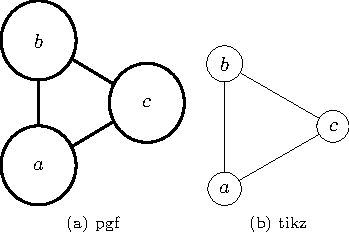
\includegraphics{pdf/pgftikzsimple}
\end{figure}

However, the main difference is in the generated code. Here is the \texttt{pgf} output:
\begin{quote}{\ttfamily \raggedright \noindent
{\%}~Edge:~a~-{}-~b~\\
{\textbackslash}draw~{[}{]}~(19bp,38bp)~-{}-~(19bp,60bp);~\\
{\%}~Edge:~b~-{}-~c~\\
{\textbackslash}draw~{[}{]}~(35bp,70bp)~-{}-~(55bp,58bp);~\\
{\%}~Edge:~c~-{}-~a~\\
{\textbackslash}draw~{[}{]}~(55bp,40bp)~-{}-~(35bp,28bp);~\\
{\%}~Node:~a~\\
{\textbackslash}begin{\{}scope{\}}~\\
{\textbackslash}pgfsetstrokecolor{\{}black{\}}~\\
{\textbackslash}draw~(19bp,19bp)~ellipse~(18bp~and~19bp);~\\
{\textbackslash}draw~(19bp,19bp)~node~{\{}{\$}a{\$}{\}};~\\
{\textbackslash}end{\{}scope{\}}~\\
{\%}~Node:~b~\\
{\textbackslash}begin{\{}scope{\}}~\\
{\textbackslash}pgfsetstrokecolor{\{}black{\}}~\\
{\textbackslash}draw~(19bp,79bp)~ellipse~(18bp~and~19bp);~\\
{\textbackslash}draw~(19bp,79bp)~node~{\{}{\$}b{\$}{\}};~\\
{\textbackslash}end{\{}scope{\}}~\\
{\%}~Node:~c~\\
{\textbackslash}begin{\{}scope{\}}~\\
{\textbackslash}pgfsetstrokecolor{\{}black{\}}~\\
{\textbackslash}draw~(71bp,49bp)~ellipse~(18bp~and~19bp);~\\
{\textbackslash}draw~(71bp,49bp)~node~{\{}{\$}c{\$}{\}};~\\
{\textbackslash}end{\{}scope{\}}
}\end{quote}

Compare the above code with the \texttt{tikz} output:
\begin{quote}{\ttfamily \raggedright \noindent
{\textbackslash}node~(a)~at~(19bp,19bp)~{[}draw,circle,{]}~{\{}{\$}a{\$}{\}};~\\
{\textbackslash}node~(b)~at~(19bp,79bp)~{[}draw,circle,{]}~{\{}{\$}b{\$}{\}};~\\
{\textbackslash}node~(c)~at~(71bp,49bp)~{[}draw,circle,{]}~{\{}{\$}c{\$}{\}};~\\
{\textbackslash}draw~{[}{]}~(a)~-{}-~(b);~\\
{\textbackslash}draw~{[}{]}~(b)~-{}-~(c);~\\
{\textbackslash}draw~{[}{]}~(c)~-{}-~(a);
}\end{quote}

The code is much more compact and it is quite easy to modify the graph.


%___________________________________________________________________________

\hypertarget{the-dot2texi-latex-package}{}
\pdfbookmark[1]{The dot2texi LaTeX package}{the-dot2texi-latex-package}
\subsection*{The dot2texi LaTeX package}
\label{the-dot2texi-latex-package}

The dot2texi package allows you to embed DOT graphs directly in you LaTeX document. The package will automatically run \texttt{dot2tex} for you and include the generated code. Example:
\begin{quote}{\ttfamily \raggedright \noindent
{\textbackslash}documentclass{\{}article{\}}~\\
{\textbackslash}usepackage{\{}dot2texi{\}}~\\
~\\
{\textbackslash}usepackage{\{}tikz{\}}~\\
{\textbackslash}usetikzlibrary{\{}shapes,arrows{\}}~\\
~\\
{\textbackslash}begin{\{}document{\}}~\\
{\textbackslash}begin{\{}dot2tex{\}}{[}neato,options=-tmath{]}~\\
digraph~G~{\{}~\\
~~~~node~{[}shape="circle"{]};~\\
~~~~a{\_}1~->~a{\_}2~->~a{\_}3~->~a{\_}4~->~a{\_}1;~\\
~~~~{\}}~\\
{\textbackslash}end{\{}dot2tex{\}}~\\
~\\
{\textbackslash}end{\{}document{\}}
}\end{quote}

When the above code is run through LaTeX, the following will happen is shell escape is enabled:
\begin{itemize}
\item {} 
The graph is written to file.

\item {} 
\texttt{dot2tex} is run on the DOT file.

\item {} 
The generated code is included in the document.

\end{itemize}

The whole process is completely automated. The generated graph will look like this:
\begin{figure}[H]
\centering

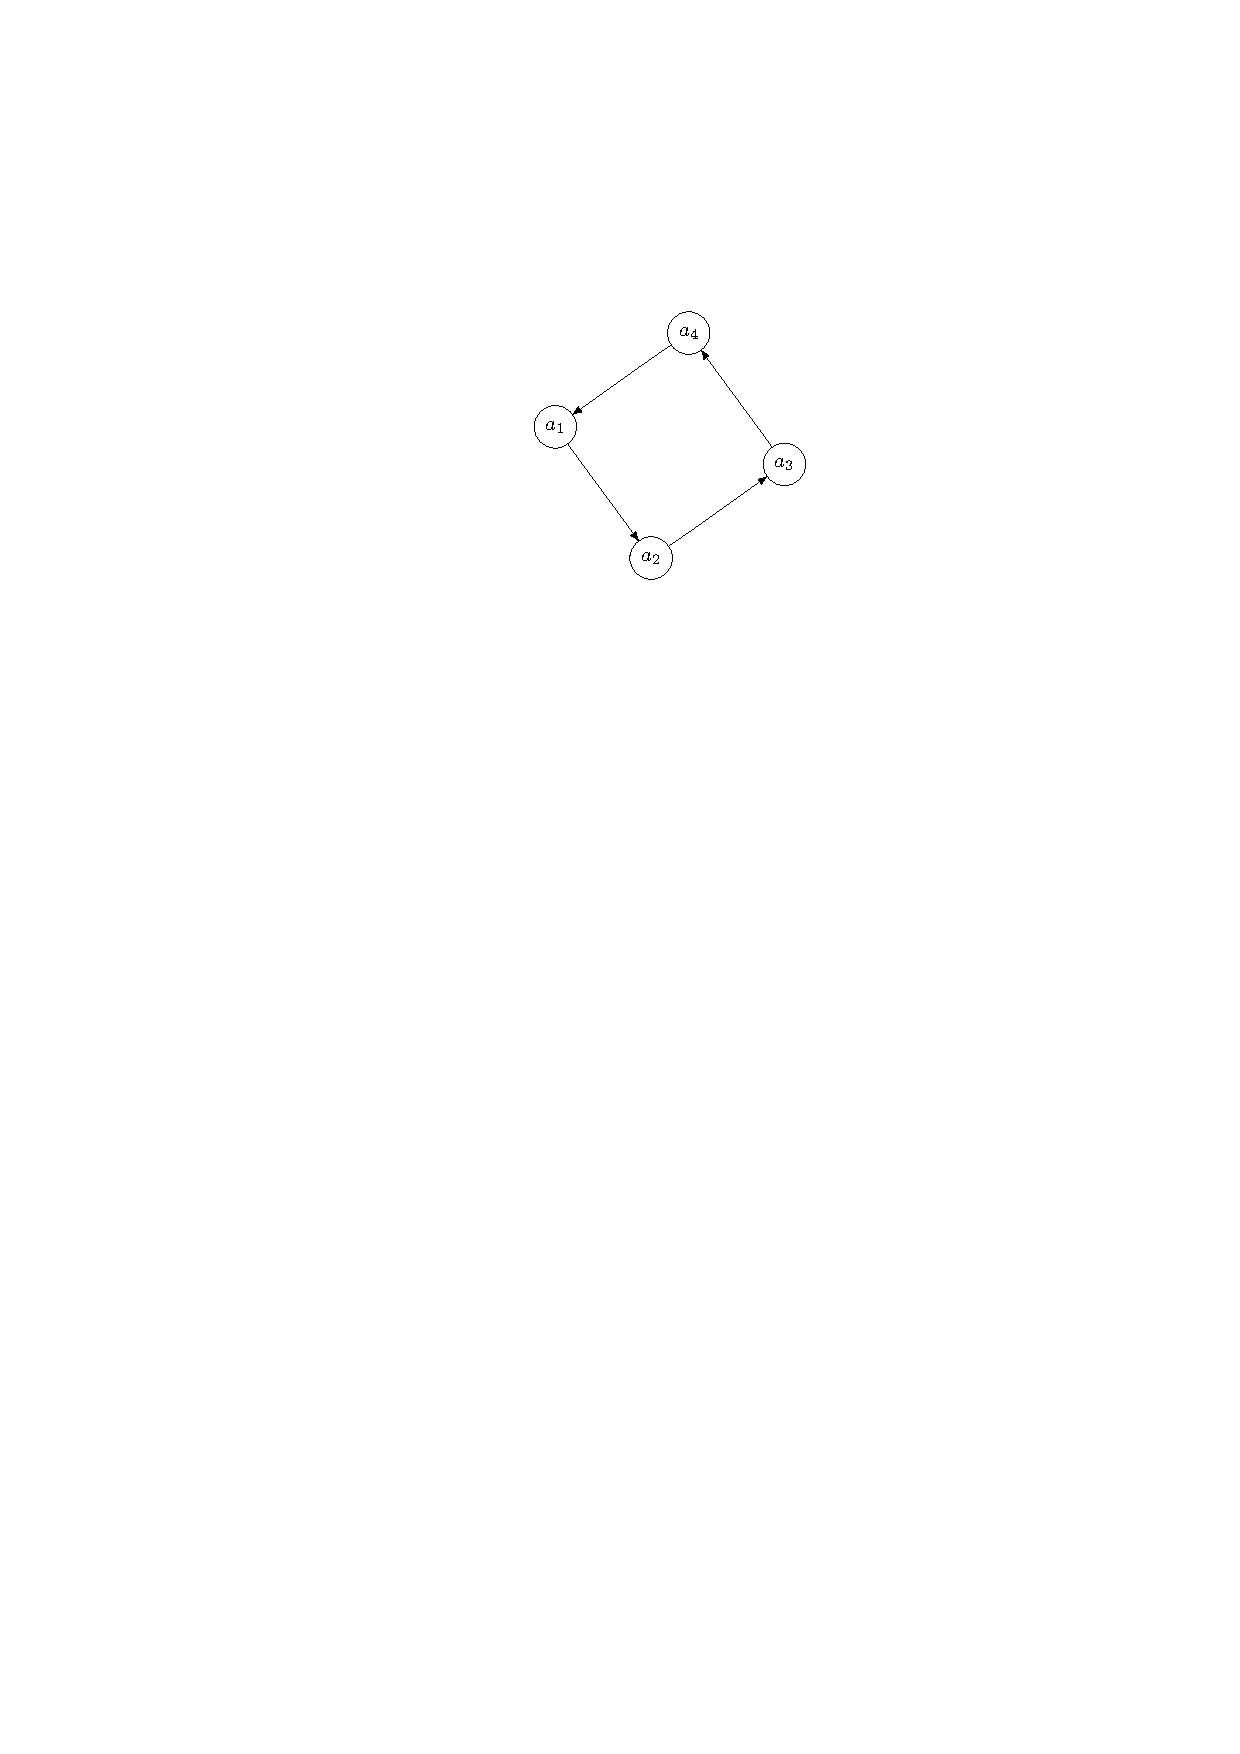
\includegraphics{pdf/dot2texiex1}
\end{figure}

The \texttt{codeonly} option is useful in conjunction with \texttt{dot2texi}, especially when used with the \texttt{tikz} output format. Here is an example that shows how to annotate a graph:
\begin{quote}{\ttfamily \raggedright \noindent
{\textbackslash}documentclass{\{}article{\}}~\\
{\textbackslash}usepackage{\{}tikz{\}}~\\
{\textbackslash}usetikzlibrary{\{}arrows,shapes{\}}~\\
{\textbackslash}usepackage{\{}dot2texi{\}}~\\
{\textbackslash}begin{\{}document{\}}~\\
{\%}~Define~layers~\\
{\textbackslash}pgfdeclarelayer{\{}background{\}}~\\
{\textbackslash}pgfdeclarelayer{\{}foreground{\}}~\\
{\textbackslash}pgfsetlayers{\{}background,main,foreground{\}}~\\
~\\
{\%}~The~scale~option~is~useful~for~adjusting~spacing~between~nodes.~\\
{\%}~Note~that~this~works~best~when~straight~lines~are~used~to~connect~\\
{\%}~the~nodes.~\\
{\textbackslash}begin{\{}tikzpicture{\}}{[}>=latex',scale=0.8{]}~\\
~~~~{\%}~set~node~style~\\
~~~~{\textbackslash}tikzstyle{\{}n{\}}~=~{[}draw,shape=circle,minimum~size=2em,~\\
~~~~~~~~~~~~~~~~~~~~~~~~inner~sep=0pt,fill=red!20{]}~\\
~~~~{\textbackslash}begin{\{}dot2tex{\}}{[}dot,tikz,codeonly,styleonly,options=-s~-tmath{]}~\\
~~~~~~~~digraph~G~~{\{}~\\
~~~~~~~~~~~~node~{[}style="n"{]};~\\
~~~~~~~~~~~~A{\_}1~->~B{\_}1;~A{\_}1~->~B{\_}2;~A{\_}1~->~B{\_}3;~\\
~~~~~~~~~~~~B{\_}1~->~C{\_}1;~B{\_}1~->~C{\_}2;~\\
~~~~~~~~~~~~B{\_}2~->~C{\_}2;~B{\_}2~->~C{\_}3;~\\
~~~~~~~~~~~~B{\_}3~->~C{\_}3;~B{\_}3~->~C{\_}4;~\\
~~~~~~~~{\}}~\\
~~~~{\textbackslash}end{\{}dot2tex{\}}~\\
~~~~{\%}~annotations~\\
~~~~{\textbackslash}node{[}left=1em{]}~at~(C{\_}1.west)~~(l3)~{\{}Level~3{\}};~\\
~~~~{\textbackslash}node~at~(l3~|-~B{\_}1)~(l2){\{}Level~2{\}};~\\
~~~~{\textbackslash}node~at~(l3~|-~A{\_}1)~(l1)~{\{}Level~1{\}};~\\
~~~~{\%}~Draw~lines~to~separate~the~levels.~First~we~need~to~calculate~\\
~~~~{\%}~where~the~middle~is.~\\
~~~~{\textbackslash}path~(l3)~-{}-~coordinate~(l32)~(l2)~-{}-~coordinate~(l21)~(l1);~\\
~~~~{\textbackslash}draw{[}dashed{]}~(C{\_}1~|-~l32)~-{}-~(l32~-|~C{\_}4);~\\
~~~~{\textbackslash}draw{[}dashed{]}~(C{\_}1~|-~l21)~-{}-~(l21~-|~C{\_}4);~\\
~~~~{\textbackslash}draw{[}<->,red{]}~(A{\_}1)~to{[}out=-120,in=90{]}~(C{\_}2);~\\
~~~~{\%}~Highlight~the~A{\_}1~->~B{\_}1~->~C{\_}2~path.~Use~layers~to~draw~\\
~~~~{\%}~behind~everything.~\\
~~~~{\textbackslash}begin{\{}pgfonlayer{\}}{\{}background{\}}~\\
~~~~~~~~{\textbackslash}draw{[}rounded~corners=2em,line~width=3em,blue!20,cap=round{]}~\\
~~~~~~~~~~~~~~~~(A{\_}1.center)~-{}-~(B{\_}1.west)~-{}-~(C{\_}2.center);~\\
~~~~{\textbackslash}end{\{}pgfonlayer{\}}~\\
{\textbackslash}end{\{}tikzpicture{\}}~\\
{\textbackslash}end{\{}document{\}}
}\end{quote}
\begin{figure}[H]
\centering

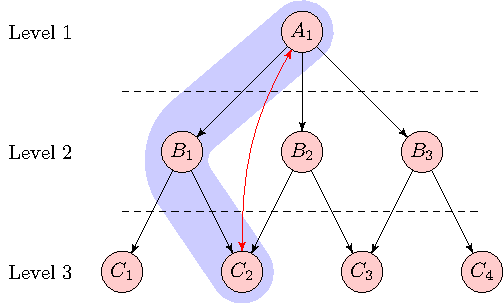
\includegraphics{pdf/dot2texiex2}
\end{figure}

\end{document}
